% =====================================================================
% Tarea 2 CIT3435 — Resiliencia de la red de fibra óptica chilena ante el 27F
% Plantilla oficial IEEEtran (conference). Paper corto (5–6 páginas), en español.
% Compilar: latexmk -pdf main.tex   (pdfLaTeX + BibTeX)
% =====================================================================
\documentclass[conference]{IEEEtran}
\IEEEoverridecommandlockouts
\usepackage[utf8]{inputenc}
\usepackage[T1]{fontenc}
\usepackage[spanish,es-tabla,es-nodecimaldot,es-noshorthands]{babel}
\usepackage{cite}
\usepackage{amsmath,amssymb,amsfonts}
\usepackage{graphicx}
\graphicspath{{figuras/}}
\usepackage{booktabs}
\usepackage{siunitx}
\sisetup{output-decimal-marker={,}, group-separator={.}, group-minimum-digits=4, group-digits=integer}
\usepackage{listings}
\usepackage{upquote}
\renewcommand{\lstlistingname}{Código}
\lstset{basicstyle=\ttfamily\scriptsize, breaklines=true, columns=fullflexible, frame=single, captionpos=b, aboveskip=6pt, belowskip=4pt, belowcaptionskip=4pt, framesep=3pt, xleftmargin=0pt, xrightmargin=0pt, showstringspaces=false}
\usepackage{textcomp}
\usepackage{xcolor}
\usepackage{url}
\newcommand{\pendiente}[1]{\textcolor{red}{[PENDIENTE: #1]}}
\newcommand{\attr}{\mathrm{ATTR}}

\begin{document}

\title{Resiliencia de la red de fibra óptica chilena ante el terremoto del 27F:
confiabilidad promedio entre pares de nodos clave}

\author{\IEEEauthorblockN{Benjamín Morales}
\IEEEauthorblockA{\textit{Escuela de Informática y Telecomunicaciones} \\
\textit{Universidad Diego Portales}, Santiago, Chile}
}

\maketitle

\begin{abstract}
Se evalúa cuánto se degrada la conectividad entre los nodos clave de la Internet chilena frente a un sismo como el del 27 de febrero de 2010.
Con el archivo de infraestructura que SUBTEL entregó a partir del Estudio de NIC Chile se construye una topología con PostGIS y pgRouting, se identifican 24 nodos que generan, intercambian o reciben información y se calcula la confiabilidad promedio entre pares (ATTR).
El sismo se obtiene del catálogo del USGS y la probabilidad de falla de cada enlace se estima desde el epicentro con una atenuación de aceleración chilena y una tasa de cortes por kilómetro.
Con solo la fibra detectada el ATTR baja de 0,217 a 0,132 y, al sumar postes, caminos y ferry como enlaces sintéticos, de 1,000 a 0,314.
La zona entre Talca y Concepción queda desconectada del resto del país.
El repositorio reproduce todas las cifras con un solo comando.
\end{abstract}

\begin{IEEEkeywords}
resiliencia de redes, fibra óptica, terremoto, confiabilidad entre pares, pgRouting
\end{IEEEkeywords}

% ---------------------------------------------------------------------
\section{Introducción}
\label{sec:intro}
Internet es infraestructura crítica y su continuidad depende de pocos enlaces físicos.
El terremoto del 27 de febrero de 2010 dejó a más del \SI{60}{\percent} de la Internet chilena desconectada alrededor de seis horas, por fallas de interconexión y respaldo en Santiago, y cortó fibras que iban en puentes derribados \cite{niclabs2018}.

Este trabajo estima cuánto se degrada la conectividad entre los nodos que generan, intercambian y reciben información si un sismo como el 27F afectara la infraestructura de fibra hoy reportada.
La métrica es la confiabilidad promedio entre pares (ATTR) \cite{boettcher2018} y la amenaza es un modelo probabilístico de falla por enlace derivado del epicentro.
En este trabajo se construye una topología de red en PostGIS y pgRouting con el archivo de infraestructura entregado por SUBTEL, se modela la probabilidad de falla de cada enlace con parámetros tomados de la literatura y se calcula el ATTR antes y después del sismo en dos escenarios de red.
Todo queda en un repositorio que se ejecuta con un solo comando e incluye un mapa Leaflet.

% ---------------------------------------------------------------------
\section{Entorno y datos}
\label{sec:datos}
Todo se ejecuta en contenedores Docker sobre Ubuntu (x86\_64, 3 núcleos, \SI{10}{GB}): PostgreSQL 16.9 con PostGIS 3.5.2 y pgRouting 3.8.0, y Python 3.12 con psycopg, pyshp, numpy, scipy, networkx y folium, de versiones fijadas en \texttt{requirements.txt}.
Se fija pgRouting 3.8.0 porque es la última versión con \texttt{pgr\_createTopology}, declarada obsoleta en esa versión y eliminada en la serie 4 \cite{pgrouting38}.

La infraestructura es el archivo que SUBTEL entregó (carta ORD.~7479/G) en respuesta a la solicitud de acceso a la información AN002T0005610, con cuatro capas lineales en WGS84 derivadas del Estudio de NIC Chile \cite{niclabs2018,subtel2023saip}.
El sismo se descargó del servicio FDSN del USGS por su identificador \texttt{official20100227063411530\_30} \cite{usgs2010maule}, y la métrica se toma de Boettcher et al. \cite{boettcher2018}.

El archivo SAIP suma \num{4497} líneas y \SI{27523,0}{km}, cifra consistente con los \SI{28000}{km} que declara la carta (Tabla~\ref{tab:capas}).
Solo la fibra, con \SI{10312,8}{km}, es tendido detectado y equivale a \SI{37}{\percent} del total y a los \SI{10342}{km} del Cuadro~4.1 del Estudio; las otras tres capas son rutas donde no se verificó fibra y se tratan como enlaces sintéticos.
El levantamiento es de 2016 a 2018 y se hizo desde caminos públicos, no distingue tendido aéreo de soterrado, no incluye los anillos urbanos y el atributo \texttt{id} se repite (\num{1482} identificadores para \num{1915} líneas de fibra). La red analizada es entonces la reportada hoy y no la de 2010.

\begin{table}[t]
\centering
\caption{Capas del archivo SAIP; solo la fibra es tendido detectado y el resto se marca como sintético.}
\label{tab:capas}
\footnotesize
\begin{tabular}{@{}lrrc@{}}
\toprule
Capa & Líneas & km & Sintética \\
\midrule
Fibra óptica & \num{1915} & \num{10312,8} & no \\
Postación eléctrica & \num{1213} & \num{6712,4} & sí \\
Caminos sin postación & \num{1165} & \num{8107,7} & sí \\
Ferry & \num{204} & \num{2390,1} & sí \\
\bottomrule
\end{tabular}
\end{table}

% ---------------------------------------------------------------------
\section{Nodos clave}
\label{sec:nodos}
Un nodo clave es un punto de la red que genera, intercambia o recibe información.
Generan contenido y servicios los centros de datos (G), intercambian tráfico entre redes los puntos de intercambio, IXP (I), y reciben tráfico del exterior o lo entregan a la población los aterrizajes de cables submarinos, el cruce terrestre a Argentina y las capitales regionales, que actúan como nodos troncales (R).
El criterio sigue al Estudio, según el cual la red se conecta al exterior por cables submarinos y por la salida terrestre hacia Argentina, con anillos en Santiago, Valparaíso, Temuco y Concepción \cite{niclabs2018}.
Las instalaciones y sus coordenadas provienen de PeeringDB \cite{peeringdb} y los aterrizajes de submarinecablemap \cite{submarinecablemap}, que ubica los cables internacionales en Arica (SAm-1, Prat y SPCS/Mistral) y Valparaíso (SAm-1, SAC, Curie, Prat y SPCS/Mistral); solo SAm-1 y SAC operaban en 2010.
Las coordenadas de Iquique, Antofagasta y La Serena (fuente C en la Tabla~\ref{tab:nodos}) son aterrizajes del cable nacional Prat, y la de Punta Arenas, de Fibra Óptica Austral; ambos cables entraron en servicio en 2020, después del sismo y del levantamiento de los datos.
Se definen 24 nodos y 276 pares (Tabla~\ref{tab:nodos}): 10 generan, 6 intercambian y 17 reciben, y Santiago, Concepción y Temuco reúnen varios roles porque coinciden varias instalaciones.
Cada nodo se ubica en la topología mediante su vértice.
Rapa Nui queda fuera por no tener conexión terrestre con el continente.

\begin{table*}[t]
\centering
\caption{Nodos clave: rol (G genera, I intercambia, R recibe), fuente de la coordenada (P PeeringDB, C submarinecablemap, A aproximada), vértice en la topología y ubicación (latitud, longitud).}
\label{tab:nodos}
\scriptsize
\setlength{\tabcolsep}{3pt}
\begin{tabular}{@{}llccrrrllccrrr@{}}
\toprule
Id & Nodo & Rol & F. & Vért. & Lat. & Lon. & Id & Nodo & Rol & F. & Vért. & Lat. & Lon. \\
\midrule
N01 & Arica & R & C & 4588 & $-18{,}473$ & $-70{,}307$ & N13 & DC Pudahuel & G & P & 40 & $-33{,}448$ & $-70{,}848$ \\
N02 & Iquique & R & C & 4589 & $-20{,}217$ & $-70{,}142$ & N14 & Rancagua & R & A & 42 & $-34{,}171$ & $-70{,}744$ \\
N03 & Antofagasta & R & C & 4590 & $-23{,}650$ & $-70{,}400$ & N15 & Talca & R & A & 48 & $-35{,}426$ & $-71{,}655$ \\
N04 & Copiapó & R & A & 4591 & $-27{,}367$ & $-70{,}332$ & N16 & Chillán & R & A & 50 & $-36{,}606$ & $-72{,}103$ \\
N05 & La Serena & R & C & 4592 & $-29{,}906$ & $-71{,}250$ & N17 & Concepción & R,I,G & P & 52 & $-36{,}816$ & $-73{,}048$ \\
N06 & Valparaíso & R & C & 4593 & $-33{,}046$ & $-71{,}621$ & N18 & Temuco & R,I,G & P & 57 & $-38{,}743$ & $-72{,}596$ \\
N07 & MetroPort Viña & I & P & 4594 & $-33{,}029$ & $-71{,}567$ & N19 & Valdivia & R,I & A & 60 & $-39{,}814$ & $-73{,}246$ \\
N08 & DC Scala Placilla & G & P & 4536 & $-33{,}136$ & $-71{,}558$ & N20 & DC Osorno & G & P & 62 & $-40{,}591$ & $-72{,}953$ \\
N09 & Los Andes (cruce) & R & A & 4579 & $-32{,}834$ & $-70{,}598$ & N21 & Puerto Montt & R,G & P & 65 & $-41{,}468$ & $-72{,}940$ \\
N10 & Santiago Centro & R,I,G & P & 130 & $-33{,}444$ & $-70{,}656$ & N22 & Coyhaique & R & A & 68 & $-45{,}571$ & $-72{,}069$ \\
N11 & DC Santiago Norte & G & P & 135 & $-33{,}357$ & $-70{,}699$ & N23 & Punta Arenas & R & C & 70 & $-53{,}167$ & $-70{,}933$ \\
N12 & DC Lampa & G & P & 137 & $-33{,}297$ & $-70{,}702$ & N24 & PatagoniaIX y DC & I,G & P & 72 & $-53{,}047$ & $-70{,}873$ \\
\bottomrule
\end{tabular}
\end{table*}

% ---------------------------------------------------------------------
\section{Topología}
\label{sec:topologia}
Los cuatro shapefiles se cargan con pyshp en una tabla única con la capa de cada línea y su marca de sintética.
Las líneas se parten en cada cruce exacto con \texttt{ST\_UnaryUnion}, que además disuelve los tramos solapados, y resultan \num{4766} aristas.
Este paso reemplaza a \texttt{pgr\_nodeNetwork}, que se intentó primero y aborta con \emph{Splitter line has linear intersection with input} sobre la red completa y sobre las capas de fibra y de caminos por separado.
Cada arista hereda la capa de mayor prioridad que la cubre (fibra, postación, caminos, ferry), por lo que la fibra conserva sus \SI{10312,8}{km}.

La topología se construye con \texttt{pgr\_createTopology} (Código~\ref{lst:topologia}), que asigna un vértice a cada extremo y une los separados por menos que la tolerancia.
Se usa \ang{0,0001} en WGS84, unos \SI{11}{m} (tercera fila de la Tabla~\ref{tab:tolerancia}).
Un barrido de cinco tolerancias entre \SI{1}{m} y \SI{111}{m} lo respalda: desde \SI{5}{m} los componentes de la fibra se estabilizan en 125, de modo que esa escala une desajustes de digitalización sin fusionar tramos realmente separados.
La tabla de vértices tiene \num{4572} filas y, tras agregar las acometidas, \num{4594}; el Código~\ref{lst:topologia} muestra el resultado de la llamada y un extracto de esa tabla. La columna \texttt{prob\_falla} de la tabla de aristas vale 0 en las \num{4766} aristas, que es el estado de operación.

\begin{lstlisting}[language=SQL,caption={Topología (resultado OK) y extracto de la tabla de vértices, con los vértices de los primeros nodos clave.},label={lst:topologia}]
SELECT pgr_createTopology('red_noded', 0.0001,
  'the_geom', 'id', 'source', 'target', clean := true);
 pgr_createtopology
--------------------
 OK

SELECT v.id, n.nombre, grado, lon, lat
FROM red_noded_vertices_pgr v
JOIN nodos_clave n ON n.vertice_id = v.id LIMIT 3;
  id  |   nombre    | grado |   lon    |   lat
------+-------------+-------+----------+----------
 4588 | Arica       |     1 | -70.3067 | -18.4734
 4589 | Iquique     |     3 | -70.1422 | -20.2167
 4590 | Antofagasta |     1 | -70.4000 | -23.6500
\end{lstlisting}

\begin{table}[t]
\centering
\caption{Efecto de la tolerancia en la topología; los componentes de la fibra (RF) se estabilizan en 125.}
\label{tab:tolerancia}
\footnotesize
\begin{tabular}{@{}rrrr@{}}
\toprule
Tolerancia (m) & Vértices & Comp. RF & Comp. RE \\
\midrule
1,1 & \num{4589} & 128 & 33 \\
5,5 & \num{4577} & 125 & 31 \\
11,1 & \num{4572} & 125 & 31 \\
55,5 & \num{4556} & 125 & 30 \\
111,0 & \num{4521} & 125 & 28 \\
\bottomrule
\end{tabular}
\end{table}

La fibra queda dividida en 125 componentes, 44 de ellos de una sola arista (\SI{180,8}{km}), y los cuatro mayores, de \num{1944,4}, \num{1085,9}, \num{1055,0} y \SI{1050,3}{km}, son bloques regionales sin continuidad entre sí; la red con las cuatro capas tiene 31 componentes, dos de los cuales reúnen \SI{26921,8}{km}, al norte y al sur de Santiago.
\texttt{pgr\_analyzeGraph} detecta 348 extremos libres, 10 segmentos aislados y 20 posibles brechas, sin intersecciones sin nodar.
Estas limitaciones vienen de los datos (\SI{10313}{km} de fibra frente a cerca de \SI{28000}{km} recorridos), por lo que se evalúan dos escenarios con el mismo procedimiento: RF, solo con la fibra detectada, y RE, que agrega postes, caminos y ferry como enlaces sintéticos.

Como los anillos urbanos no se levantaron \cite{niclabs2018}, cada nodo se une con un segmento recto al vértice más cercano de cada componente de fibra situada a menos de \SI{20}{km}, que representa el punto de presencia donde se interconectan los tendidos de una ciudad; \SI{20}{km} es del orden del radio del Gran Santiago.
Se agregan 57 acometidas, de \SI{477,6}{km} en total y \SI{8,4}{km} en promedio, marcadas como sintéticas.
Ningún nodo queda sin cobertura, y como no hay componentes sin fibra a menos de \SI{20}{km} de un nodo, todas las acometidas se enganchan a fibra.
Con ellas, los 24 nodos quedan en 10 componentes en RF y en una sola en RE.

% ---------------------------------------------------------------------
\section{Métrica y modelo de falla}
\label{sec:modelo}

\subsection{Confiabilidad promedio entre pares}
Sea $S=\{s_1,\dots,s_K\}$ el conjunto de nodos clave y $p_e$ la probabilidad de falla del enlace $e$.
La confiabilidad promedio entre pares (\emph{average two-terminal reliability}, ATTR) es la fracción esperada de pares de nodos clave que permanecen conectados \cite{rai1990,boettcher2018,neumayer2010}:
\begin{equation}
\attr = \binom{K}{2}^{-1} \sum_{i<j} \Pr\left[ s_i \leftrightarrow s_j \right].
\label{eq:attr}
\end{equation}
Con $p_e=0$ la conectividad es determinista y la ecuación~\eqref{eq:attr} es exacta: si los grupos de nodos conectados tienen $n_g$ nodos, $\attr=\sum_g \binom{n_g}{2}\binom{K}{2}^{-1}$.
Con probabilidades positivas, el cálculo exacto exige enumerar los $2^{|E|}$ estados de los enlaces y se estima por Monte Carlo \cite{boettcher2018}, con $Z_{ij}^{(n)}=1$ si $s_i$ y $s_j$ quedan conectados en la realización $n$, en la que cada enlace funciona con probabilidad $1-p_e$ de forma independiente:
\begin{equation}
\widehat{\attr} = \frac{1}{N}\sum_{n=1}^{N} \binom{K}{2}^{-1} \sum_{i<j} Z_{ij}^{(n)}.
\label{eq:mc}
\end{equation}
Cada término de la suma exterior está en $[0,1]$, por lo que el error estándar es a lo más $0{,}5/\sqrt{N}=0{,}005$ con $N=\num{10000}$; ese valor de $N$ se elige por esa cota, y se informa también el intervalo de confianza de \SI{95}{\percent}.
La semilla es fija (\texttt{20100227}) para que las cifras sean reproducibles.
El script \texttt{src/attr.py} lee de la base de datos las columnas \texttt{source}, \texttt{target} y \texttt{prob\_falla} de cada enlace y el vértice de cada nodo, y calcula las componentes conexas con \texttt{scipy}.
El efecto del sismo se mide como la diferencia entre el ATTR posterior y el anterior.

\subsection{El sismo del 27 de febrero de 2010}
El evento se obtuvo del USGS en GeoJSON mediante una consulta que fija su identificador y el formato \cite{usgs2010maule}; la búsqueda por fecha y magnitud mínima 8 entrega solo ese evento.
El archivo se versiona sin modificar y \texttt{src/cargar\_sismo.py} lo carga en la tabla \texttt{sismo}, donde el epicentro es un punto PostGIS construido con las coordenadas del archivo (Tabla~\ref{tab:sismo}).

\begin{table}[t]
\centering
\caption{Tabla \texttt{sismo} tras cargar el GeoJSON del USGS.}
\label{tab:sismo}
\footnotesize
\begin{tabular}{@{}cccc@{}}
\toprule
Magnitud & Fecha y hora (UTC) & Prof. (km) & Epicentro (lon, lat) \\
\midrule
8,8 Mww & 2010-02-27 06:34:11,53 & 22,9 & $(-72{,}898;\,-36{,}122)$ \\
\bottomrule
\end{tabular}
\end{table}

\subsection{Probabilidad de falla de un enlace}
Cada enlace se parte en tramos $k$ de a lo más \SI{1}{km}.
La distancia hipocentral $r_k$ se calcula entre el hipocentro y el punto medio del tramo, con la distancia geodésica $d_k$ en metros sobre el elipsoide (\texttt{ST\_Distance} con \texttt{geography}, no en grados) y la profundidad $h$ del evento (ecuación~\eqref{eq:r}).
La aceleración máxima del suelo se estima con la atenuación para sismos interplaca chilenos de Saragoni et al., calibrada con roca y suelo duro \cite{saragoni2004} (ecuación~\eqref{eq:pga}), con $M_s$ igual al menor valor entre la magnitud del evento y 8,5, la magnitud de diseño interplaca de ese estudio, porque la fórmula usa ondas superficiales y estas saturan.
La tasa de cortes por kilómetro es la curva de daño en tuberías de Isoyama et al. \cite{isoyama2000} (ecuación~\eqref{eq:rr}), nula bajo el umbral $\alpha_0$.
Como los cortes ocurren de forma independiente a lo largo del enlace, el número de cortes sigue un proceso de Poisson y el enlace falla si ocurre al menos uno (ecuación~\eqref{eq:pe}).
El Código~\ref{lst:prob} muestra la consulta que lo aplica a cada enlace y actualiza la columna \texttt{prob\_falla}.
La Tabla~\ref{tab:parametros} da el valor y el origen de cada parámetro y la Fig.~\ref{fig:modelo} el resultado: a \SI{100}{km} del epicentro la aceleración es \SI{538}{cm/s^2} y la tasa \SI{0,22}{cortes/km}, y a \SI{300}{km}, \SI{199}{cm/s^2} y \SI{0,012}{cortes/km}.
\begin{lstlisting}[float=t,language=SQL,caption={Probabilidad de falla por enlace (extracto simplificado de \texttt{sql/05\_probabilidades.sql}); las distancias se calculan en metros con \texttt{geography}.},label={lst:prob}]
WITH q AS (SELECT geom, profundidad_km h,
           LEAST(mag, par('ms_max')) ms FROM sismo),
tramos AS (SELECT e.id, s.geom g FROM red_noded e,
  LATERAL ST_DumpSegments(ST_Segmentize(
    e.the_geom::geography, 1000)::geometry) s),
calc AS (SELECT t.id, ST_Length(t.g::geography)/1000 l_km,
  sqrt(power(ST_Distance(
    ST_LineInterpolatePoint(t.g, 0.5)::geography,
    q.geom::geography)/1000, 2) + power(q.h, 2)) r_km,
  q.ms FROM tramos t, q),
agg AS (SELECT id, sum(tasa_cortes_km(
    pga_cms2(r_km, ms)) * l_km) lam FROM calc GROUP BY id)
UPDATE red_noded e SET prob_falla = 1 - exp(-a.lam)
FROM agg a WHERE a.id = e.id;
\end{lstlisting}

\begin{align}
r_k &= \sqrt{d_k^2 + h^2}, \label{eq:r}\\
\alpha(r_k) &= \frac{A\, e^{C M_s}}{(r_k + D)^{B}}, \label{eq:pga}\\
R(\alpha) &= C_p C_d C_g\, c\, (\alpha - \alpha_0)^{b}, \quad \alpha > \alpha_0, \label{eq:rr}\\
p_e &= 1 - \exp\Big(-\sum_{k \in e} R(\alpha(r_k))\, \ell_k\Big). \label{eq:pe}
\end{align}

\begin{table}[t]
\centering
\caption{Parámetros del modelo de falla y su fuente.}
\label{tab:parametros}
\footnotesize
\begin{tabular}{@{}p{1.45cm}p{2.0cm}p{3.75cm}@{}}
\toprule
Parámetro & Valor & Fuente \\
\midrule
$h$, $M_w$ & \SI{22,9}{km}, 8,8 & Tabla~\ref{tab:sismo} (USGS) \\
$M_s$ & 8,5 & Magnitud de diseño interplaca \cite{saragoni2004} \\
$A$, $C$, $D$, $B$ & 1,995; 1,283; \SI{30}{km}; 1,086 & \cite{saragoni2004}, Tabla 1, ec.~(2): interplaca, roca y suelo duro \\
$\alpha_0$ & \SI{100}{cm/s^2} & \cite{isoyama2000}: aceleración desde la que hay daño \\
$c$, $b$ & \num{2,88e-6}; 1,97 & \cite{isoyama2000}, ec.~(5): curva estándar \\
$C_p$, $C_d$, $C_g$ & 0,3; 1,6; 1,0 & \cite{isoyama2000}, Tabla 3: material dúctil, diámetro \SI{75}{mm}, terreno aluvial \\
Ferry & $p_e=0$ & Sin tendido terrestre expuesto \\
\bottomrule
\end{tabular}
\end{table}

\begin{figure*}[t]
\centering
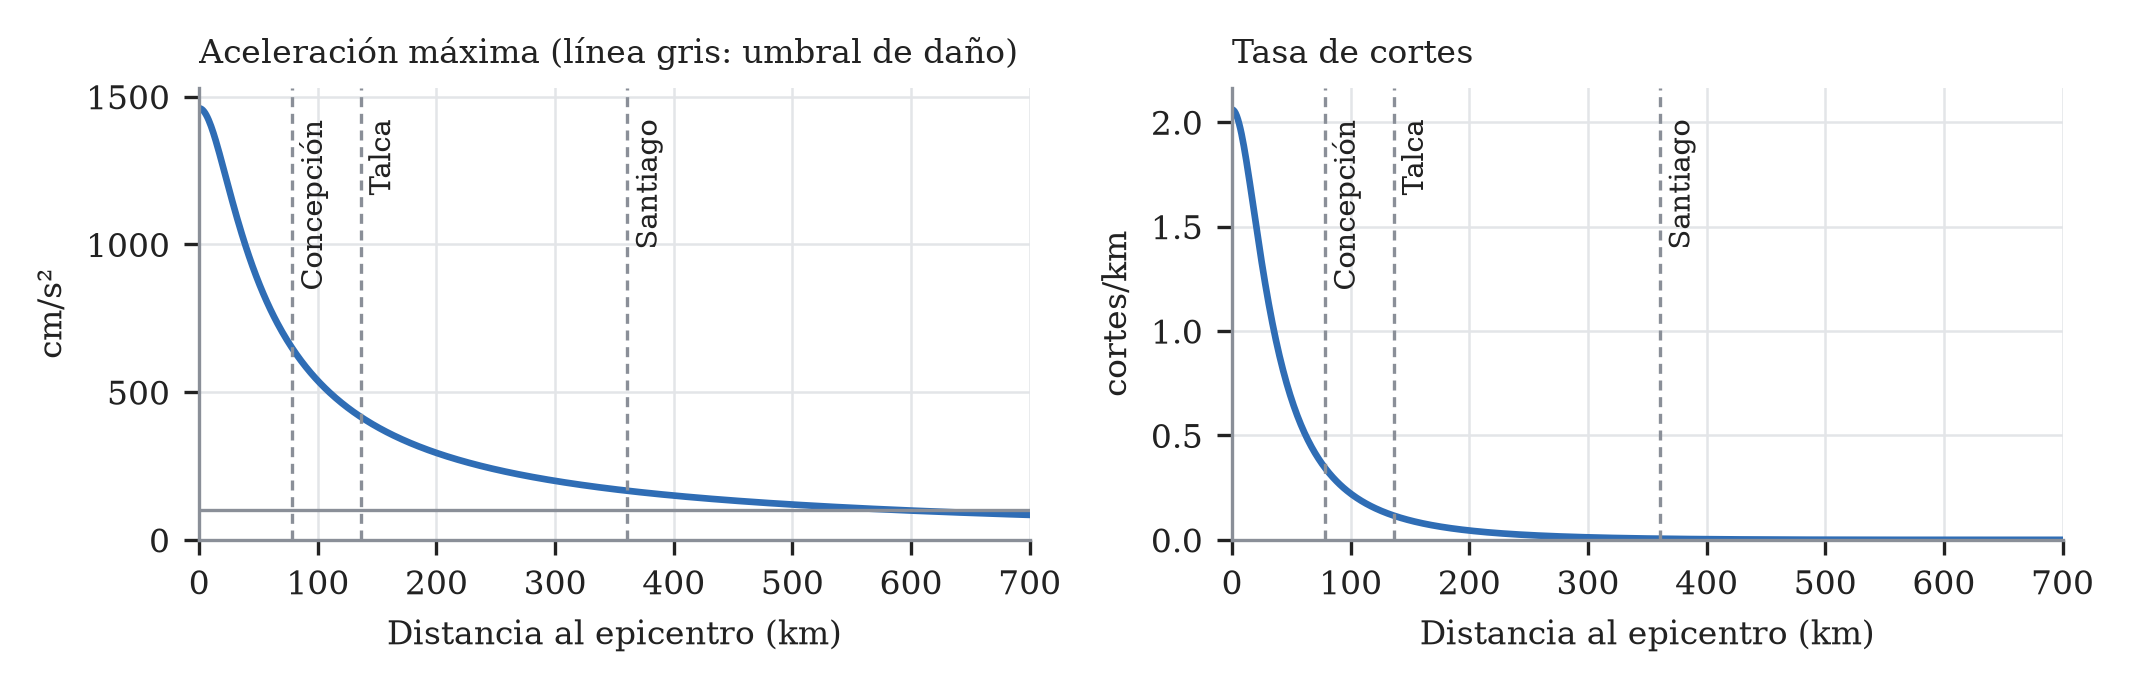
\includegraphics[width=0.78\textwidth]{modelo_pga.png}
\caption{Aceleración máxima (izquierda) y tasa de cortes (derecha) según la distancia al epicentro, con $M_s=8{,}5$ y $h=\SI{22,9}{km}$. Las líneas verticales marcan Concepción, Talca y Santiago, y la horizontal gris, el umbral de daño. La tasa de cortes es despreciable más allá de unos \SI{300}{km}.}
\label{fig:modelo}
\end{figure*}

La adaptación de la curva de tuberías a la fibra se apoya en tres razones.
Kongar et al. estiman para cables enterrados tasas de reparación de Poisson similares a las de las tuberías \cite{kongar2017}.
Con Poisson, la supervivencia del enlace es el exponente de la suma de las tasas sobre su largo y no depende de cómo la topología lo divide en tramos.
El umbral $\alpha_0$ cumple el papel de la intensidad mínima de daño que Valentini et al. fijan para sus enlaces \cite{valentini2019}, aquí con daño gradual y no como salto.
Los factores se eligen para un cable continuo y delgado: $C_p=0{,}3$ es el del hierro dúctil, el material más flexible de la tabla de Isoyama et al., que no tabulan un factor para fibra, por lo que se adopta por analogía y se evalúa en la sensibilidad; $C_d=1{,}6$ corresponde al menor diámetro y $C_g=1$ al terreno aluvial sin licuefacción.
Las acometidas se modelan como cualquier tramo terrestre y el ferry tiene $p_e=0$.
La fibra chilena es principalmente aérea \cite{niclabs2018} y el modelo no representa de forma directa los cortes en puentes ni por deformación del suelo.

% ---------------------------------------------------------------------
\section{Resultados}
\label{sec:resultados}

\begin{figure*}[t]
\centering
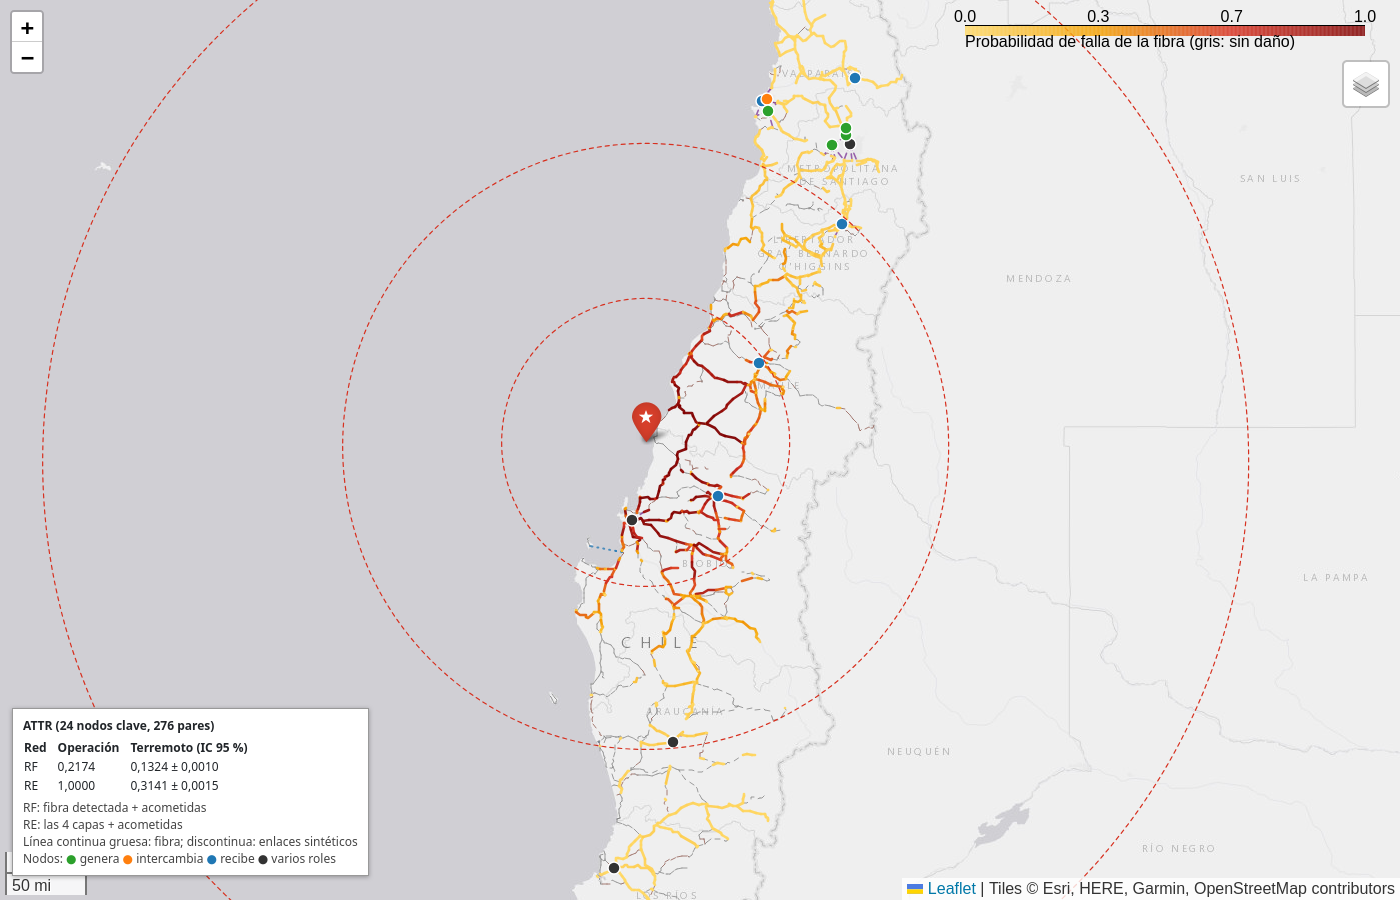
\includegraphics[width=0.86\textwidth]{mapa_centro_sur.png}
\caption{Captura del mapa Leaflet del centro-sur de Chile. La fibra se colorea de amarillo a rojo oscuro según su probabilidad de falla y en gris cuando no hay daño; las líneas discontinuas son enlaces sintéticos y los círculos rojos, la aceleración de 400, 200 y 100 cm/s$^2$ del modelo. El daño se concentra entre Talca y Concepción, a unos 80--140 km del epicentro (estrella).}
\label{fig:mapa}
\end{figure*}

\subsection{ATTR en operación}
Con todos los enlaces en servicio, el ATTR de RE es \num{1,000}: los 24 nodos forman una componente y los 276 pares están conectados.
El de RF es \num{0,217}, igual a $60/276$, porque los nodos se reparten en grupos de 11 (Copiapó a Rancagua, con Valparaíso y Santiago), 3 (Talca, Chillán y Concepción), 2 (Osorno y Puerto Montt), 2 (Punta Arenas) y seis nodos aislados: Arica, Iquique, Antofagasta, Temuco, Valdivia y Coyhaique.
Una consulta independiente en SQL con \texttt{pgr\_connectedComponents} reproduce ambos valores.
Las brechas entre grupos son cortas en varios casos: Valdivia queda a \SI{1,1}{km} de Osorno, el grupo de Santiago a \SI{4,1}{km} del de Talca y Temuco a \SI{13,2}{km} del de Chillán, lo que indica tramos no levantados; las mayores, con Arica a \SI{183,2}{km} de Iquique y Punta Arenas a \SI{552,5}{km} de Coyhaique, reflejan que el extremo sur no tiene fibra terrestre continua en los datos y que hoy se une por el cable submarino Fibra Óptica Austral, de 2020.
El ATTR de RF es por tanto una cota inferior de la conectividad real y el de RE una cota superior, y concuerda con el diagnóstico del Estudio de que la red de fibra no es conexa \cite{niclabs2018}.

\subsection{Probabilidades de falla}
El modelo asigna probabilidad positiva a \num{2290} de las \num{4823} aristas y a \num{1310} de las \num{2066} de fibra, \num{212} de ellas con probabilidad mayor que 0,5.
De los \SI{10313}{km} de fibra, \SI{4516}{km} (\SI{44}{\percent}) no sufren daño y \SI{484}{km} fallan con probabilidad mayor que 0,9; todas las probabilidades están en $[0,1]$ y el daño llega hasta \SI{594}{km} del epicentro.
Los enlaces más afectados están a menos de \SI{65}{km} del epicentro y los menos afectados a más de \SI{576}{km} (Tabla~\ref{tab:enlaces}).
Las probabilidades quedan guardadas en \texttt{prob\_falla} y se exportan en \texttt{main.sql}.

Como contraste con datos reales, el acelerógrafo del Colegio Concepción, en San Pedro de la Paz, registró \SI{594}{cm/s^2} y \SI{638}{cm/s^2} en sus dos componentes horizontales \cite{usgsnsmp2010}, y el modelo da \SI{626}{cm/s^2} en ese punto, a \SI{82}{km} del epicentro.
En los nodos clave da \SI{650}{cm/s^2} en Concepción, \SI{416}{cm/s^2} en Talca y \SI{166}{cm/s^2} en Santiago.

\begin{table}[t]
\centering
\caption{Enlaces de fibra más afectados (arriba) y menos afectados (abajo): largo, distancia al epicentro, aceleración máxima, cortes esperados $\lambda$ y probabilidad de falla.}
\label{tab:enlaces}
\footnotesize
\begin{tabular}{@{}rrrrrr@{}}
\toprule
Enlace & km & Dist. (km) & PGA (cm/s$^2$) & $\lambda$ & $p_e$ \\
\midrule
1262 & 12,6 & 33 & \num{1071} & 12,3 & 1,000 \\
1153 & 10,3 & 37 & \num{1020} & 9,7 & 1,000 \\
1710 & 23,1 & 63 & 753 & 9,4 & 1,000 \\
\midrule
736 & 6,1 & 594 & 100 & $<10^{-8}$ & $<0{,}001$ \\
611 & 9,9 & 593 & 100 & $10^{-7}$ & $<0{,}001$ \\
3024 & 10,7 & 590 & 101 & $1{,}3\times10^{-6}$ & $<0{,}001$ \\
\bottomrule
\end{tabular}
\end{table}

\subsection{ATTR tras el terremoto}
El ATTR cae de \num{0,217} a \num{0,132} en RF y de \num{1,000} a \num{0,314} en RE, una diferencia de \num{-0,085} (\SI{-39,1}{\percent}) y de \num{-0,686} (\SI{-68,6}{\percent}), con errores estándar menores que \num{0,001} (Tabla~\ref{tab:attr} y Código~\ref{lst:attr}).
La caída se concentra en el corredor Maule--Biobío: Talca, Chillán y Concepción quedan sin conexión con ningún otro nodo en RE, y Temuco y los nodos al sur conservan solo conexiones entre sí (Tabla~\ref{tab:nodos_afectados}).
La probabilidad de que Santiago esté conectado con Concepción, Talca o Temuco es 0 en las \num{10000} realizaciones, y con Valparaíso baja a \num{0,611} en RE.

\begin{lstlisting}[caption={Extracto de la salida de \texttt{src/attr.py}; el terremoto usa Monte Carlo con $N=10000$ y semilla 20100227.},label={lst:attr}]
[RF] operacion: ATTR = 0.2174  exacto (p = 0)
[RE] operacion: ATTR = 1.0000  exacto (p = 0)
[RF] terremoto: ATTR = 0.1324  IC95 0.1314-0.1334
[RE] terremoto: ATTR = 0.3141  IC95 0.3126-0.3157
\end{lstlisting}

\begin{table}[t]
\centering
\caption{ATTR antes y después del terremoto ($N=\num{10000}$).}
\label{tab:attr}
\footnotesize
\begin{tabular}{@{}lcccc@{}}
\toprule
Red & Operación & Terremoto (IC 95 \%) & Dif. & Var. \\
\midrule
RF & \num{0,217} & \num{0,132} (\num{0,1314}--\num{0,1334}) & \num{-0,085} & \SI{-39,1}{\percent} \\
RE & \num{1,000} & \num{0,314} (\num{0,3126}--\num{0,3157}) & \num{-0,686} & \SI{-68,6}{\percent} \\
\bottomrule
\end{tabular}
\end{table}

\begin{table}[t]
\centering
\caption{Conectividad media de cada nodo con los demás, antes y después del terremoto.}
\label{tab:nodos_afectados}
\footnotesize
\begin{tabular}{@{}lcccc@{}}
\toprule
 & \multicolumn{2}{c}{RF} & \multicolumn{2}{c}{RE} \\
\cmidrule(lr){2-3}\cmidrule(lr){4-5}
Nodo & Antes & Después & Antes & Después \\
\midrule
Talca, Chillán, Concepción & 0,087 & 0,000 & 1,000 & 0,000 \\
Temuco & 0,000 & 0,000 & 1,000 & 0,171 \\
Valdivia & 0,000 & 0,000 & 1,000 & 0,237 \\
Osorno a Punta Arenas & 0,043 & 0,042 & 1,000 & 0,244 \\
Rancagua & 0,435 & 0,177 & 1,000 & 0,345 \\
Santiago Centro & 0,435 & 0,315 & 1,000 & 0,454 \\
\bottomrule
\end{tabular}
\end{table}

Los enlaces críticos se identifican con los puentes del grafo en operación, agrupados por los pares de nodos que separan.
En RE, el corredor de mayor riesgo, de 19 aristas de fibra y \SI{107,4}{km} cerca de Santiago, aísla a Valparaíso, Viña del Mar y Placilla del resto (separa \SI{22,8}{\percent} de los pares) con probabilidad de falla \num{0,376}.
Le sigue uno de 5 aristas y \SI{48,1}{km} que separa a los nodos del norte, de Arica a La Serena, y a Los Andes del resto (\SI{39,1}{\percent} de los pares, probabilidad \num{0,141}).
Estos corredores están a más de \SI{360}{km} del epicentro y no explican la caída principal, que viene de la zona del epicentro, donde varias rutas alternativas tienen probabilidad cercana a 1.

La conclusión cualitativa se mantiene en la sensibilidad (Tabla~\ref{tab:sensibilidad}).
Con $M_s=8{,}8$ el ATTR de RE baja a \num{0,127} y con $C_p=1$, a \num{0,183}; exponer o no las acometidas al sismo cambia el resultado en menos de \num{0,003}.
En cambio, $D_{\max}$ afecta el estado en operación: con \SI{10}{km} RE no es conexa (\num{0,438}), por lo que su valor depende de que los puntos de presencia unan tendidos a esa escala.

\begin{table}[t]
\centering
\caption{Sensibilidad del ATTR a las decisiones del modelo.}
\label{tab:sensibilidad}
\footnotesize
\begin{tabular}{@{}lcccc@{}}
\toprule
Caso & RF oper. & RF terr. & RE oper. & RE terr. \\
\midrule
Base & \num{0,217} & \num{0,132} & \num{1,000} & \num{0,314} \\
$M_s=8{,}8$ & \num{0,217} & \num{0,042} & \num{1,000} & \num{0,127} \\
$C_p=1$ & \num{0,217} & \num{0,064} & \num{1,000} & \num{0,183} \\
Acometidas sin falla & \num{0,217} & \num{0,134} & \num{1,000} & \num{0,316} \\
$D_{\max}=\SI{10}{km}$ & \num{0,065} & \num{0,045} & \num{0,438} & \num{0,230} \\
$D_{\max}=\SI{30}{km}$ & \num{0,236} & \num{0,157} & \num{1,000} & \num{0,352} \\
\bottomrule
\end{tabular}
\end{table}

\subsection{Mapa}
La Fig.~\ref{fig:mapa} muestra el mapa Leaflet generado por \texttt{src/mapa.py} a partir de la base de datos, con la fibra coloreada por probabilidad de falla, los enlaces sintéticos en trazo discontinuo, los nodos clave por rol, el epicentro y los círculos de aceleración del modelo; el mapa interactivo (\texttt{mapa/index.html}) incluye además el detalle de cada enlace y nodo.


% ---------------------------------------------------------------------
\section{Discusión}
\label{sec:discusion}
El modelo concentra el daño en Maule y Biobío, la zona donde el Estudio reporta fibras cortadas en puentes derribados durante el 27F \cite{niclabs2018}.
Sin embargo, Kwasinski observó relativamente poco daño en la infraestructura de telecomunicaciones que registró y halló la mayoría de los postes dañados en zonas de tsunami \cite{kwasinski2010}; el modelo podría entonces sobrestimar los cortes en una red aérea y flexible, aun con el factor de material bajo que adopta.
La mayor interrupción del 27F, de más del \SI{60}{\percent} de la Internet por unas seis horas, se debió a fallas de interconexión y respaldo dentro de Santiago \cite{niclabs2018}, es decir, a la capa lógica, que un ATTR sobre la red física no captura; en el modelo Santiago recibe solo \SI{166}{cm/s^2}.
La restauración de las telecomunicaciones estuvo además acoplada con la de la energía eléctrica \cite{duenas2012}, factor que tampoco se modela.

Las limitaciones del modelo son varias.
La fuente es un punto en el epicentro, aunque la ruptura fue extensa, lo que subestima el daño en los extremos; se usa la mediana de la atenuación sin dispersión y se extrapola más allá de los eventos de calibración de la fórmula, que llegan a $M_s=7{,}8$ \cite{saragoni2004}; se aplica una curva de tuberías a un cable; los enlaces fallan de forma independiente; y no hay tsunami, licuefacción, puentes ni energía.
La coincidencia con el acelerógrafo de Concepción es un solo punto y no valida la atenuación en toda la red.
La red es la de 2016 a 2018, sin capa lógica ni anillos urbanos, y no incluye el cable submarino Fibra Óptica Austral, que hoy conecta el extremo sur.
Los postes y caminos de RE no garantizan fibra, por lo que RF y RE acotan el resultado real.

% ---------------------------------------------------------------------
\section{Conclusiones}
\label{sec:conclusiones}
Con la infraestructura reportada, un sismo como el 27F reduce el ATTR de \num{0,217} a \num{0,132} (\SI{-39,1}{\percent}) solo con la fibra detectada y de \num{1,000} a \num{0,314} (\SI{-68,6}{\percent}) al sumar los enlaces sintéticos.
El efecto principal es el aislamiento del corredor Talca--Concepción y del sur respecto de Santiago, porque todas las rutas entre ellos cruzan la zona de mayor aceleración.
Que RF sea de solo \num{0,217} sin sismo muestra que los datos disponibles no garantizan la conectividad de los nodos clave, y los resultados dependen sobre todo de la magnitud, del factor de material y del radio de las acometidas.
El trabajo futuro es modelar la ruptura extensa y la capa lógica de interconexión.

\section*{Disponibilidad}
El código, \texttt{main.sql} y el mapa están en \url{https://github.com/benjamin09111/tarea2-resiliencia}.
El archivo \texttt{main.sql} es un volcado de la base de datos con la infraestructura (aristas y vértices), los nodos clave, el sismo, los parámetros del modelo y la columna \texttt{prob\_falla} ya calculada, y se carga en una base vacía.
Desde un clon limpio, \texttt{python3 main.py} levanta la base con Docker, carga \texttt{main.sql}, recalcula la topología, las probabilidades y el ATTR antes y después del sismo, comprueba que coinciden con este artículo y sirve el mapa Leaflet.
El \texttt{README} detalla las dependencias y cada cifra del artículo proviene de la carpeta \texttt{resultados/}.

% Bibliografía incluida en el propio archivo (generada con IEEEtran.bst a partir de referencias.bib
% con BibTeX), para que main.tex compile con pdfLaTeX sin BibTeX ni archivos adicionales.
% Generated by IEEEtran.bst, version: 1.14 (2015/08/26)
\begin{thebibliography}{10}
\providecommand{\url}[1]{#1}
\csname url@samestyle\endcsname
\providecommand{\newblock}{\relax}
\providecommand{\bibinfo}[2]{#2}
\providecommand{\BIBentrySTDinterwordspacing}{\spaceskip=0pt\relax}
\providecommand{\BIBentryALTinterwordstretchfactor}{4}
\providecommand{\BIBentryALTinterwordspacing}{\spaceskip=\fontdimen2\font plus
\BIBentryALTinterwordstretchfactor\fontdimen3\font minus
  \fontdimen4\font\relax}
\providecommand{\BIBforeignlanguage}[2]{{%
\expandafter\ifx\csname l@#1\endcsname\relax
\typeout{** WARNING: IEEEtran.bst: No hyphenation pattern has been}%
\typeout{** loaded for the language `#1'. Using the pattern for}%
\typeout{** the default language instead.}%
\else
\language=\csname l@#1\endcsname
\fi
#2}}
\providecommand{\BIBdecl}{\relax}
\BIBdecl

\bibitem{niclabs2018}
\BIBentryALTinterwordspacing
{NIC Chile Research Labs}, ``Estudio y recomendaciones sobre la resiliencia de
  la infraestructura de la internet chilena,'' Universidad de Chile, Informe
  técnico final, versión 2.0, Dec. 2018, proyecto InnovaChile--CORFO
  15BPE-47225, encargado por la Subsecretaría de Telecomunicaciones. [Online].
  Available:
  \url{https://www.nic.cl/estudios/resiliencia_uchile_corfo_subtel.pdf}
\BIBentrySTDinterwordspacing

\bibitem{boettcher2018}
N.~Boettcher, Y.~Prieto, S.~E. Restrepo, and J.~E. Pezoa, ``Resilient
  multiculture network design in the presence of exploit-triggered correlated
  failures,'' \emph{IEEE Latin America Transactions}, vol.~16, no.~9, pp.
  2336--2343, 2018.

\bibitem{pgrouting38}
\BIBentryALTinterwordspacing
{pgRouting Contributors}, \emph{pgRouting Manual, versión 3.8:
  pgr\_createTopology (deprecada desde v3.8.0)}, 2025. [Online]. Available:
  \url{https://docs.pgrouting.org/3.8/en/pgr_createTopology.html}
\BIBentrySTDinterwordspacing

\bibitem{subtel2023saip}
{Subsecretaría de Telecomunicaciones}, ``Respuesta a solicitud de acceso a la
  información pública {AN002T0005610} ({ORD.} {N}$^\circ$ 7479/{G}), archivo
  ``respuesta\_t5610'','' Santiago, Chile, May 2023.

\bibitem{usgs2010maule}
\BIBentryALTinterwordspacing
{U.S. Geological Survey}, ``M 8.8 -- 2010 {Maule}, {Chile} earthquake (evento
  official20100227063411530\_30),'' ANSS Comprehensive Earthquake Catalog
  (ComCat), servicio FDSN, 2010. [Online]. Available:
  \url{https://earthquake.usgs.gov/fdsnws/event/1/query?eventid=official20100227063411530_30&format=geojson}
\BIBentrySTDinterwordspacing

\bibitem{peeringdb}
\BIBentryALTinterwordspacing
{PeeringDB}, ``Internet exchanges and facilities in {Chile},'' API pública,
  consultas \texttt{ix?country=CL}, \texttt{fac?country=CL} e \texttt{ixfac}.
  [Online]. Available: \url{https://www.peeringdb.com}
\BIBentrySTDinterwordspacing

\bibitem{submarinecablemap}
\BIBentryALTinterwordspacing
{TeleGeography}, ``Submarine cable map: landing points in {Chile},'' API v3,
  \texttt{landing-point-geo.json}. [Online]. Available:
  \url{https://www.submarinecablemap.com}
\BIBentrySTDinterwordspacing

\bibitem{rai1990}
S.~Rai and D.~P. Agrawal, \emph{Distributed Computing Network
  Reliability}.\hskip 1em plus 0.5em minus 0.4em\relax IEEE Computer Society
  Press, 1990.

\bibitem{neumayer2010}
S.~Neumayer and E.~Modiano, ``Network reliability with geographically
  correlated failures,'' in \emph{Proceedings of IEEE INFOCOM 2010}, 2010, pp.
  1--9.

\bibitem{saragoni2004}
\BIBentryALTinterwordspacing
G.~R. Saragoni, M.~Astroza, and S.~Ruiz, ``Comparative study of subduction
  earthquake ground motion of north, central and south america,'' in
  \emph{Proceedings of the 13th World Conference on Earthquake Engineering},
  no. 104, Vancouver, Canada, 2004. [Online]. Available:
  \url{https://www.iitk.ac.in/nicee/wcee/article/13_104.pdf}
\BIBentrySTDinterwordspacing

\bibitem{isoyama2000}
\BIBentryALTinterwordspacing
R.~Isoyama, E.~Ishida, K.~Yune, and T.~Shirozu, ``Seismic damage estimation
  procedure for water supply pipelines,'' in \emph{Proceedings of the 12th
  World Conference on Earthquake Engineering}, no. 1762, Auckland, New Zealand,
  2000. [Online]. Available:
  \url{https://www.iitk.ac.in/nicee/wcee/article/1762.pdf}
\BIBentrySTDinterwordspacing

\bibitem{kongar2017}
I.~Kongar, S.~Giovinazzi, and T.~Rossetto, ``Seismic performance of buried
  electrical cables: Evidence-based repair rates and fragility functions,''
  \emph{Bulletin of Earthquake Engineering}, vol.~15, pp. 3151--3181, 2017.

\bibitem{valentini2019}
A.~Valentini, B.~Vass, J.~Oostenbrink, L.~Cs{\'a}k, F.~Kuipers, B.~Pace,
  D.~Hay, and J.~Tapolcai, ``Network resiliency against earthquakes,'' in
  \emph{Proc. 11th International Workshop on Resilient Networks Design and
  Modeling (RNDM)}, 2019.

\bibitem{usgsnsmp2010}
\BIBentryALTinterwordspacing
{U.S. Geological Survey, National Strong-Motion Project}, ``Preliminary
  corrected peak ground acceleration and velocity and pseudo-spectral
  acceleration values for the {February} 27, 2010, offshore {Maule}, {Chile}
  earthquake,'' Tabla de valores registrados, publicada el 5 de mayo de 2010,
  2010. [Online]. Available:
  \url{https://escweb.wr.usgs.gov/nsmp-data/recent_events/20100227_0634_peaks_files/sheet001.html}
\BIBentrySTDinterwordspacing

\bibitem{kwasinski2010}
\BIBentryALTinterwordspacing
A.~Kwasinski, ``M 8.8 {Maule}, {Chile} earthquake of 2010,'' Registro
  fotográfico de daños, The University of Texas at Austin, 2010. [Online].
  Available: \url{https://users.ece.utexas.edu/~kwasinski/chile2010.html}
\BIBentrySTDinterwordspacing

\bibitem{duenas2012}
L.~Due{\~n}as-Osorio and A.~Kwasinski, ``Quantification of lifeline system
  interdependencies after the 27 {February} 2010 {$M_w$} 8.8 offshore {Maule},
  {Chile}, earthquake,'' \emph{Earthquake Spectra}, vol.~28, no.~S1, pp.
  S581--S603, 2012.

\end{thebibliography}

\end{document}
